\documentclass[11pt]{article}
\usepackage[letterpaper,margin=0.94in]{geometry}
\usepackage{amsmath,amssymb,amsthm,mathtools,booktabs,tabularx,graphicx}
\usepackage{xcolor,microtype,fancyhdr}
\usepackage[colorlinks=true,linkcolor=blue!45!black,citecolor=blue!45!black,urlcolor=blue!45!black]{hyperref}
\usepackage{bookmark}
\setlength{\emergencystretch}{1.5em}
\setlength{\parskip}{0.25em}
\newtheorem{theorem}{Theorem}[section]
\newtheorem{lemma}[theorem]{Lemma}
\newtheorem{corollary}[theorem]{Corollary}
\newtheorem{proposition}[theorem]{Proposition}
\theoremstyle{definition}\newtheorem{definition}[theorem]{Definition}
\theoremstyle{remark}\newtheorem{remark}[theorem]{Remark}
\newcommand{\ord}{\operatorname{ord}}
\newcommand{\m}{\mathfrak m}
\newcommand{\F}{F}
\pagestyle{fancy}
\fancyhf{}
\fancyhead[L]{\small Unequal branch data and resonant zero filters}
\fancyhead[R]{\small Research report}
\fancyfoot[C]{\thepage}
\setlength{\headheight}{14pt}
\hypersetup{pdftitle={Unequal branch data and resonant zero filters},pdfauthor={Research prepared for Vladimir Reshetnikov}}
\title{\textbf{Unequal branch data and resonant zero filters}\\[5pt]
\large Two extensions of methods in the supplied RH/GRH development}
\author{Research prepared for Vladimir Reshetnikov}
\date{27 November 2026}
\begin{document}
\maketitle
\begin{abstract}
We prove two results suggested by the specific local and analytic mechanisms
of the supplied Lean development and its accompanying collection of research
reports. First, we solve the unequal-precision branch-recovery problem over
an arbitrary coefficient field, explicitly asked in the article. We determine
the exact adversarial distance of a formal-series jet, reduce every extremal
ambiguity to a product of observed branch equations, give a finite tree
algorithm, and find the unique componentwise minimum precision vector attaining
maximum distance. A separate sufficient condition yields a decoder using two
linear systems. Second, we classify the shortest positive measure annihilating
two distinct positive real frequencies. Its optimal support has an asymmetric cube-root
cusp at every odd integer ratio $m\ge3$, and we determine the exact first-order cost of
shortening that support. Complete proofs, exact finite-field checks, numerical
illustrations, and a formalization plan are included. The two main theorems
are unconditional; RH/Dirichlet GRH identifies the critical-line modes to which
the positive filters apply. Novelty is established relative to the supplied
article; global priority is not claimed, and substantial classical antecedents
are explicitly credited.
\end{abstract}
\setcounter{tocdepth}{1}
\hypersetup{bookmarksdepth=2}
\tableofcontents
\newpage

\section{Source analysis and the precise contribution}
\label{sec:sources}

\subsection{The inspected snapshot}

The analysis uses the following immutable source versions:
\begin{center}
\begin{tabular}{ll}
\toprule
ProveIt & \texttt{2a9f8e3ee74a1824d57546f0b1b4f1cef5df93d6}\\
Vendored upstream & \texttt{72fead102f663d5c7a407964a13dc0cf9d977207}\\
\bottomrule
\end{tabular}
\end{center}
The vendor README identifies the latter as the readable edition imported
without changes. It also says that this separate Lake package was not built
as part of the ProveIt import. The article README describes a merge of 120
reports, 689 pages and 869 named results, and explicitly distinguishes that
merge from an independent mathematical review \cite{Source,Vendor}.
We retrieved the article's 21 section files, mapped their topics and theorem
headings, and read the relevant proofs in the source, branch-recovery and
positive-filter sections. This is a focused extension study, not a claim to
have independently checked all 869 results.

The short Lean files \path{src/Statements.lean} and \path{src/Main.lean}
were inspected directly. The exported statement
\path{LFunction_ne_zero_of_half_lt_re} quantifies over Dirichlet characters
and asserts nonvanishing in $\Re s>1/2$, except for the principal pole.
\path{riemannHypothesis} uses Mathlib's own RH statement; the other exports
give zeros on the line in the critical strip and the primitive special case
\cite{LeanExports}. These are the precise input theorems relevant here.
No export in those files asserts GRH for every Artin or number-field Hecke
$L$-function. This task did not rerun the Lean build or replay its kernel.

\subsection{What is transferable from the proof}

The file \path{New/Reduction/MainInequality.lean} explicitly combines
short integral forms, an index estimate, enough independent forms, and a
lower bound for the size of integral forms. Its theorem
\path{New.star_inequality} concludes, in the source's notation,
\[
 D.m\,D.totalRemainder\le D.f\,D.a\,D.logB^5.
\]
\path{New/Reduction/OneSidedBound.lean} converts that comparison into
\path{eventually_primeRemainder_le_rpow} and then \path{grh}.
The determinant proof uses local divisibility, chosen twists, and the product
formula; it supplies an arithmetic estimate before the analytic zero criterion
is applied \cite{LeanMechanism}. Merely changing the prime weight would not
supply the corresponding arithmetic construction.

At the local end, the inspected formal-group file
\path{Lib/CM/FormalGroup/InseparableDegree.lean} works with the orders of
reduced power series and includes the multiplication and substitution laws
\path{reducedOrder_mul} and \path{reducedOrder_subst}. The article's
Lubin--Tate section abstracts these local orders into contacts between branches
and reconstruction of finite jets \cite{LeanLocal,Source}. Section~2 below
extends that abstraction to different precisions and corrupted records.

At the analytic end, the article constructs positive averages on the
logarithmic scale whose transform cancels selected zero contributions.
Positivity preserves inequalities when averaging a prime statistic.
The one-frequency and consecutive-harmonic optimal-width theorems leave the
general prescribed-frequency problem open in the article. Section~3 gives
a complete two-frequency calculation and its singular perturbation laws.

\subsection{What is new relative to the article}

\begin{center}\small
\begin{tabularx}{\textwidth}{@{}p{0.24\textwidth}XX@{}}
\toprule
Topic & Already in the supplied article & Proved here\\
\midrule
Branch records & Common precision; clean thresholds with exactly $d$ branches &
Exact distance for arbitrary unequal precisions and any number of redundant branches\\
Precision allocation & Least common length at maximum distance &
Unique componentwise least vector and exact total coefficient cost\\
Error recovery & Exact uniqueness criterion and enumeration of candidate error sets &
Two linear systems under a stated stronger distance condition\\
Positive filters & One frequency with multiplicity; consecutive harmonics &
All real ratios for two frequencies, full equality classification, resonance and shortening laws\\
\bottomrule
\end{tabularx}
\end{center}

The first extension answers the unequal-length part of the article's question
\texttt{lub:q:adversarial} over a field. It leaves the question's coefficient-ring
case $\mathcal O/\pi^r$, $r>1$, and the full optimal-radius polynomial decoder
unresolved. The second extension answers its two-frequency support problem;
it does not establish additional arithmetic bounds on prime errors.
Classical $P$-orderings, interpolation decoding and positive input shaping
are antecedents, not new discoveries asserted here.

\section{Exact recovery from unequal branch records}
\label{sec:jets}
\subsection{Setup and relation to the supplied sources}

Let $F$ be any field and let $B=\{u_b:b\in I\}$ be a nonempty finite set
of distinct elements of $XF[[X]]$, with $|I|=N$. Put
\[
 v=\ord_X,\qquad s_{bc}=v(u_b-u_c)\quad(b\ne c),\qquad s_{bb}=+\infty.
\]
The finite contacts are positive integers and obey the ultrametric inequality.
For a precision vector $\mathbf n=(n_b)_{b\in I}\in\mathbb Z_{\ge0}^I$ define
\[
 \Omega_{\mathbf n}(H)_b=H(X,u_b(X))\bmod X^{n_b},\qquad
 J_d(H)=H\bmod (X,Y)^d.
\]
A record with $n_b=0$ is empty. Throughout the target order $d$ is positive.
The higher coefficients of $H\in F[[X,Y]]$ are arbitrary. Thus this is
recovery of a quotient of the source, rather than ordinary decoding of a
bounded-degree polynomial.

The supplied article~\cite{Source} proves the common-length observation kernel and distance
formula in the results labelled \texttt{lub:thm:kernel} and
\texttt{lub:thm:distance}; it gives a common-length tree recursion in
\texttt{lub:thm:dp}, and the least common precision for maximum distance in
\texttt{lub:thm:saturation}. Its question \texttt{lub:q:adversarial} asks for
unequal lengths, higher coefficient precision, and faster error-location
algorithms. For exactly $d$ branches, unequal-length clean recovery is already
covered by \texttt{lub:prop:threshold}. The present extension concerns any
number of redundant branches, arbitrary unequal lengths, and errors or
erasures. Its local setting is also obtained by reducing the Lubin--Tate
branches used by the Lean development modulo the uniformizer; there
\[
 s_{bc}=q^{v_\pi(b-c)}.
\]
No Riemann hypothesis is an assumption of any result in this section.

The immutable source versions and inspection scope are recorded in Section~\ref{sec:sources}.

\subsection{Replacing every ambiguity by branch factors}

The central observation eliminates the unknown coefficients from the
distance problem. A coefficient unit is immaterial to valuations.

\begin{lemma}[Product domination for polynomials]\label{lem:domination}
Let $0\ne P\in F[[X]][Y]$ and put
$r=\ord_{(X,Y)}P$. There are indices $c_1,\ldots,c_r\in I$, with repetitions
permitted, such that
\[
 Q(X,Y)=\prod_{j=1}^r(Y-u_{c_j}(X))
 \quad\hbox{satisfies}\quad
 v(Q(X,u_b))\ge v(P(X,u_b))\quad\hbox{for every }b\in I.
\]
The empty product for $r=0$ is $1$.
\end{lemma}

\begin{proof}
Factor $P=a(X)\prod_{j=1}^D(Y-\alpha_j)$ in a valued algebraic extension of
$F((X))$, extending the $X$-adic valuation, and count roots with multiplicity.
The weighted Gauss valuation at weight one is multiplicative and gives
\[
 r=v(a)+\sum_{j=1}^D\min(1,v(\alpha_j)).
\]
This identity needs neither separability nor a Puiseux parametrization.
For completeness, the ordinary Gauss valuation is multiplicative because,
after dividing each polynomial by a coefficient of least valuation, its
nonzero reduction over the residue field has a nonzero product. Substituting
$Y=XZ$ proves the weighted version. Factoring into linear factors then gives
the displayed identity.

Let $A$ be the multiset of roots of valuation at least one, and write
$m=|A|$. The quantity
\[
 k=r-m=v(a)+\sum_{v(\alpha_j)<1}v(\alpha_j)
\]
is an integer. It is nonnegative: the ordinary Gauss valuation of $P$ is
nonnegative, and
\[
 k=G_0(P)+\sum_{0<v(\alpha_j)<1}v(\alpha_j)\ge0.
\]
For each $\alpha\in A$ choose a branch $u_{c(\alpha)}$ maximizing
$v(u_b-\alpha)$ over the finite set $B$. The ultrametric inequality implies,
for every $b$,
\[
 v(u_b-u_{c(\alpha)})\ge
 \min\{v(u_b-\alpha),v(u_{c(\alpha)}-\alpha)\}
 =v(u_b-\alpha).
\]
Every root of valuation below one contributes exactly its own valuation to
$v(P(X,u_b))$, since $v(u_b)\ge1$. Hence
\[
 Q_0=X^k\prod_{\alpha\in A}(Y-u_{c(\alpha)})
\]
dominates $P$ on all the branches and has total order $k+m=r$.
Replace each of its $k$ factors $X$ by $Y-u_{c_0}$, for any fixed $c_0\in I$.
This cannot decrease an evaluation valuation, because all contacts are at
least one. The resulting $Q$ has exactly $r$ branch factors.
\end{proof}

\begin{corollary}[Finite-record domination for formal series]\label{cor:formal}
If $H\notin\m^d$, where $\m=(X,Y)$, then a product of exactly $d-1$ branch
factors vanishes on every record on which $H$ vanishes.
\end{corollary}

\begin{proof}
Let $r=\ord_\m H<d$ and choose an integer $L>r$ with
$L\ge\max_b n_b$. The polynomial obtained by discarding terms of total degree
at least $L$ has total order $r$ and the same records as $H$, since
$u_b\in XF[[X]]$. Apply Lemma~\ref{lem:domination}. If $r<d-1$, append any
$d-1-r$ branch factors. Their evaluation valuations are nonnegative, so
previously vanishing records still vanish. The resulting product has total
order exactly $d-1$, as its coefficient of $Y^{d-1}$ is one.
\end{proof}

\begin{remark}
A stronger domination statement for the actual valuations of a formal series
follows by formal Weierstrass preparation after extracting its largest common
power of $X$. The finite-record statement above avoids needing that theorem
and is sufficient for all the distance and algorithmic claims here.
\end{remark}

\subsection{Exact distance, all errors and all erasures}

Define the target distance
\[
 D_d(\mathbf n;B)=\min_{H\notin\m^d}
       |\{b:\Omega_{\mathbf n}(H)_b\ne0\}|.
\]
For a vector $\mathbf m=(m_c)_{c\in I}$ of nonnegative integers, define
\[
 V_b(\mathbf m)=
 \begin{cases}
 +\infty,&m_b>0,\\
 \displaystyle\sum_{c\ne b}m_cs_{bc},&m_b=0.
 \end{cases}
\]
This convention avoids expressions such as $0\cdot\infty$.

\begin{theorem}[Exact unequal-record distance]\label{thm:distance}
For every $d\ge1$ and every nonnegative precision vector,
\[
 \boxed{\quad D_d(\mathbf n;B)=N-
 \max_{\substack{m_c\in\mathbb Z_{\ge0}\\\sum_cm_c=d-1}}
    |\{b:V_b(\mathbf m)\ge n_b\}|.\quad}
\]
Every maximum supplies a minimum-distance witness
$Q=\prod_c(Y-u_c)^{m_c}$. In particular the complete distance depends only on
the contact matrix and the precision vector, not on any other branch
coefficients. If $d>N$, the distance is zero at every finite precision.
\end{theorem}

\begin{proof}
Every displayed product has total order $d-1$ and its zero records are exactly
those satisfying the displayed inequalities. Conversely
Corollary~\ref{cor:formal} replaces any series with nonzero target by such a
product without reducing its zero set. Therefore the largest possible zero
set is exactly the finite maximum. If $d>N$, use each branch at least once
and pad with repeated factors to reach $d-1$ factors; this product vanishes
on all branches.
\end{proof}

\begin{corollary}[Sharp adversarial correction criterion]\label{cor:errors}
The target jet is recoverable for every $H$, despite at most $w$ arbitrarily
corrupted records and at most $z$ flagged erased records, if and only if
\[
 2w+z<D_d(\mathbf n;B).
\]
For a fixed erasure set $E$, delete its branches and use
$2w<D_d(\mathbf n|_{I\setminus E};B\setminus E)$ instead.
If all branches are erased, a positive-order target cannot be recovered.
\end{corollary}

\begin{proof}
Two explanations of a received word differ on at most the union of their
corruption sets and the erasure set, hence on at most $2w+z$ records. If their
target jets differed, their difference would contradict the distance bound.
Conversely take a minimum-distance product witness and the zero series.
Erase at most $z$ differing positions, and divide the remaining at most
$2w$ positions into two sets of size at most $w$. A word agreeing with one
explanation on one set and the other on the second has two admissible
explanations with different target jets. The distance-zero case requires no
errors at all.
\end{proof}

Nonnegative weights $a_b$ may be assigned to records. With weighted support
in place of cardinality the same proof gives
\[
 D_d^{(a)}=\sum_ba_b-
 \max_{\sum m_c=d-1}\sum_{V_b(\mathbf m)\ge n_b}a_b.
\]
For arbitrary indivisible weights the simple inequality $2w+z<D_d^{(a)}$ is
a sufficient correction condition; its necessity needs an actual partition
of differing weights into the permitted error budgets. We do not assert the
unweighted necessity proof for arbitrary weights.

\subsection{A contact-tree algorithm with explicit witnesses}

Represent the contacts by the usual rooted tree. For at least two leaves,
the root has incoming length $\ell_{\rm root}=\min_{b\ne c}s_{bc}$.
Children separate where the contact becomes larger; an internal node's
incoming length is its contact level minus its parent's level. The path
shared by two distinct leaves has total length $s_{bc}$. Terminal edges
may be assigned zero length; a mark at a leaf contributes infinity to that
leaf itself. Compress nodes with one child, leaving $O(N)$ nodes.

Let $B_v$ be the leaves below a node $v$. For $j\ge0$ and $t\ge0$ let
$A_v(j,t)$ be the largest total weight of leaves whose precision is met by
placing exactly $j$ marks in $B_v$, with repeats allowed, when contributions
from marks outside $B_v$ and from higher path segments already equal $t$ at
every leaf below $v$.

\begin{theorem}[Unequal-precision tree recursion]\label{thm:tree}
At a leaf $b$,
\[
 A_b(j,t)=\begin{cases}a_b,&j>0\text{ or }t\ge n_b,\\0,&\text{otherwise}.
 \end{cases}
\]
At an internal node with children $c$,
\[
 \boxed{\quad A_v(j,t)=
 \max_{\substack{j_c\ge0\\\sum_cj_c=j}}
       \sum_c A_c(j_c,t+j\ell_v).\quad}
\]
Consequently $D_d^{(a)}=\sum_ba_b-A_{\rm root}(d-1,0)$.
For integer contacts and precisions, the table through $j=d-1$ can be
computed in $O(Nd^2(n_{\max}+1))$ arithmetic operations, where
$n_{\max}=\max_b n_b$. Backtracking gives the mark multiplicities and thus
an explicit ambiguity witness.
\end{theorem}

\begin{proof}
All $j$ marks below an internal node share its incoming segment with every
leaf below that node. They therefore add $j\ell_v$ to the inherited value.
Once the marks are split among the children, no additional contribution
passes between distinct children; the remaining choices are independent.
At a leaf, a mark makes the polynomial vanish identically there, while an
unmarked leaf has precisely its inherited valuation. These facts prove the
recursion and its agreement with Theorem~\ref{thm:distance}.

Cap every state $t\ge n_{\max}$ at $n_{\max}$; all such leaves are already
covered. For each fixed child-input value $t'$, compute the max-convolution
\[
 C_v(j,t')=\max_{\sum j_c=j}\sum_cA_c(j_c,t')
\]
for all $j\le d-1$, then read
$A_v(j,t)=C_v(j,\min(n_{\max},t+j\ell_v))$.
The convolutions cost $O(\deg(v)d^2)$ at each $t'$, and the sum of node
degrees in a compressed tree is $O(N)$. This explains the stated bound
without an extra factor $d$ from recomputing convolutions for each state.
\end{proof}

The operation count is polynomial in the amount of observed data, and
pseudopolynomial if the lengths are supplied only in binary. The common
precision theory can also optimize by a greedy valuation sequence; unequal
leaf thresholds make the mark-allocation formulation useful.

\subsection{The unique minimum precision vector for maximum distance}

Suppose $1\le d\le N$. For each branch let $S_b(d-1)$ be the sum of its
$d-1$ largest contacts with other branches, with $S_b(0)=0$, and put
\[
 n_b^*=1+S_b(d-1).
\]

\begin{theorem}[Componentwise saturation and exact sampling cost]\label{thm:saturation}
For every precision vector,
\[
 D_d(\mathbf n;B)\le N-d+1,
\]
and equality holds if and only if $n_b\ge n_b^*$ for every $b$.
Thus $\mathbf n^*$ is the unique componentwise minimum precision vector
achieving maximum target distance. The smallest total number of recorded
field coefficients at maximum distance is exactly
\[
 \sum_bn_b^*=N+\sum_bS_b(d-1).
\]
The least common precision is $\max_bn_b^*$, so using unequal precision saves
exactly $N\max_bn_b^*-\sum_bn_b^*$ coefficients compared with the best
common-precision design.
\end{theorem}

\begin{proof}
A product of any $d-1$ distinct branch equations has total order $d-1$ and
vanishes on those $d-1$ branches, giving the upper bound.

If $n_b\le S_b(d-1)$, choose its $d-1$ highest-contact neighbours and multiply
their equations. The product vanishes on these neighbours and has valuation
$S_b(d-1)$ at $b$, so it has at least $d$ zero records and distance at most
$N-d$. This proves necessity, including $d=1$ when an empty record makes the
constant series $1$ invisible there.

For sufficiency assume all componentwise inequalities, and suppose that a
series $H$ has zero records on a $d$-element subset $S$. Divide $H$ by the
monic distinguished polynomial $\prod_{b\in S}(Y-u_b)$ to obtain a
remainder $R$ of $Y$-degree below $d$; the discarded multiple belongs to
$\m^d$. Lagrange interpolation over $F((X))$ gives
\[
 R(X,Y)=\sum_{b\in S}
 \frac{H(X,u_b)}{\prod_{c\in S\setminus\{b\}}(u_b-u_c)}
 \prod_{c\in S\setminus\{b\}}(Y-u_c).
\]
Each quotient has $X$-valuation at least
\[
 n_b-\sum_{c\in S\setminus\{b\}}s_{bc}\ge1,
\]
and each branch product has total order $d-1$. Hence $R\in\m^d$ and
$H\in\m^d$. No nonzero target can have $d$ zero records, so the distance
is at least $N-d+1$. The cost statements now follow componentwise.
\end{proof}

\begin{remark}
The sufficiency proof can avoid formal division by first truncating $H$ to
total degree at least $\max n_b$ and at least $d$, then using ordinary monic
polynomial division. Evaluation congruences and the target jet are
unchanged. Thus the formal machinery is not needed in the saturation proof
either.
\end{remark}

\paragraph{An asymmetric example.}
Over $F=\mathbb F_3$ take
\[
 B=(0,X^3,X,2X),\qquad d=2.
\]
Only the first two branches have contact $3$; all other contacts equal $1$.
The unique minimum saturation vector is
\[
 \mathbf n^*=(4,4,2,2).
\]
It records $12$ coefficients, compared with $16$ for the least common
precision, and has target distance $3$. Thus the three coefficients of
$J_2(H)$ are determined despite one arbitrarily corrupted branch record.
Reducing any one component of $\mathbf n^*$ destroys that guarantee.

More generally, over a field with at least $N-1$ elements take
$0,X^L$ and $N-2$ distinct nonzero scalar multiples of $X$, where $L>1$.
For $2\le d\le N$, the close pair has optimal precision $L+d-1$ and every
other branch has optimal precision $d$. The total is
$2L+Nd-2$, whereas common precision costs $N(L+d-1)$.
For fixed $N,d$ the ratio of common to unequal cost tends to $N/2$ as
$L\to\infty$.

\subsection{A weighted-jet extension}

Suppose, more specifically, that all $u_b\in X^\kappa F[[X]]$ for an integer
$\kappa\ge1$. Give $X$ weight one and $Y$ weight $\kappa$, and let
$J_{d,\kappa}(H)$ consist of the coefficients $[X^iY^j]H$ with
$i+\kappa j<d$. Put
\[
 k=\left\lfloor\frac{d-1}{\kappa}\right\rfloor,
 \qquad a=d-1-\kappa k,\qquad 0\le a<\kappa.
\]

\begin{corollary}[Exact distance for weighted jets]\label{cor:weighted}
Every ambiguity with nonzero $J_{d,\kappa}$ can be replaced, without losing
any zero record, by
\[
 X^a\prod_{c\in I}(Y-u_c)^{m_c},\qquad \sum_cm_c=k.
\]
Consequently its target distance is
\[
 D_{d,\kappa}(\mathbf n;B)=
 N-\max_{\sum m_c=k}|\{b:a+V_b(\mathbf m)\ge n_b\}|.
\]
The tree recursion starts with $k$ marks and inherited precision $a$.
If $k<N$, the maximum possible distance is $N-k$, and it is attained exactly
when
\[
 n_b\ge a+1+\text{the sum of the $k$ largest contacts $s_{bc}$, $c\ne b$}
 \quad\text{for every }b.
\]
If $k\ge N$, the distance is zero at every precision.
\end{corollary}

\begin{proof}
Use the weighted Gauss identity
$\ord_\kappa P=v(a_P)+\sum_\alpha\min(\kappa,v(\alpha))$
in the proof of Lemma~\ref{lem:domination}. Roots of valuation below
$\kappa$ contribute equally at every branch, while each remaining root may
be replaced by its closest branch. The resulting product of $m$ branch
factors and a power of $X$ has the same weighted order $r<d$ and dominates
the original polynomial. Multiply by $X^{d-1-r}$, and replace each group
of $\kappa$ residual factors $X$ by a branch factor. This cannot decrease
evaluation valuations, as $v(u_b-u_c)\ge\kappa$, and gives exactly the
displayed form with $k$ factors and residual exponent $a$. Truncating the
formal series at sufficiently high weighted degree justifies the same
argument for every finite collection of records.

For maximum distance, the product using $k$ distinct branches gives the
upper bound $N-k$. Necessity of each precision inequality follows by using
the $k$ closest neighbours of the branch in question and the factor $X^a$.
For sufficiency interpolate on any $k+1$ branches. The discarded full branch
product has weighted order $\kappa(k+1)\ge d$, and every Lagrange term has
weighted order at least $(a+1)+\kappa k=d$. Thus $k+1$ zero records force
the weighted target to vanish. If $k\ge N$, mark every branch and pad.
\end{proof}

\subsection{A decoder using two linear systems}

The exact distance criterion does not by itself give a polynomial-time
decoder at the entire optimal error radius. The following stronger,
computable condition does. It generalizes the error-locator linearization
behind Welch--Berlekamp decoding, while retaining the unrestricted higher
coefficients of the unknown series.

\begin{theorem}[A polynomial-time sufficient decoding condition]\label{thm:decode}
Assume arithmetic and linear algebra over $F$ are effective. Delete a known
erasure set, and retain the notation $B,\mathbf n$ for the surviving
branches and lengths. If at most $w$ remaining records are corrupted and
\[
 D_{d+w}(\mathbf n;B)>w,
\]
then $J_d(H)$ can be recovered by two finite linear systems, with no
enumeration of error sets and no factorization of an error locator. The
algorithm is polynomial in $N,n_{\max},d,w$ in field operations.
\end{theorem}

\begin{proof}
The condition implies $n_{\max}\ge d+w$: otherwise the nonzero-target series
$X^{n_{\max}}$ vanishes on every record at target order $d+w$.
Write the received record at branch $b$ as $y_b(X)$ modulo $X^{n_b}$.
Find $E,Q$ satisfying
\[
 \begin{split}
 E(X,Y)&=Y^w+\sum_{i=0}^{w-1}e_i(X)Y^i,\\
 &\hspace{-12pt}e_i(X)\in X^{w-i}F[X],\qquad
 Q\in F[X,Y],\quad\deg_{\rm total}Q<n_{\max},\\
 Q(X,u_b)&\equiv E(X,u_b)y_b(X)\pmod {X^{n_b}}\quad\text{for all }b.
 \end{split}
\]
The coefficient series $e_i$ may be truncated to terms with
$\deg_X(e_i)+i<n_{\max}$; their higher terms cannot affect any equation or
the subsequent target calculation. These are linear equations for the
unknown coefficients of $E$ and $Q$, since every $y_b$ is known, and the
coefficient of $Y^w$ in $E$ is fixed to one.

A solution exists. Let $C$ be the actual corruption set, of size at most
$w$, and take the product of $Y-u_b$ over $b\in C$, padded with arbitrary
branch factors to a monic product of degree $w$. This has the required
divisibilities. Let $Q$ be the total-degree truncation of $EH$ below
$n_{\max}$. The congruences hold on uncorrupted branches because $y_b$ is
correct, and on corrupted branches because $E$ vanishes there. Truncation
preserves the congruences. The actual locator is a formal polynomial in $Y$;
truncate its coefficients as specified above to obtain the finite $E$ in
the linear system. The omitted terms have total order at least
$n_{\max}$, so this truncation preserves both the congruences and the
required coefficient divisibilities.

Now use \emph{any} solution of the linear system, not necessarily the actual
error locator. On every uncorrupted branch the series $Q-EH$ has a zero
record, so it has at most $w$ nonzero records. By the assumed distance,
\[
 Q-EH\in\m^{d+w}.
\]
Since $E$ has total order exactly $w$, its initial homogeneous form is
nonzero in the domain $F[X,Y]$. Therefore multiplication by $E$ induces an
injective map
\[
 F[[X,Y]]/\m^d\longrightarrow
   \m^w/\m^{d+w}.
\]
Solve the second linear system
\[
 E h\equiv Q\pmod {\m^{d+w}},\qquad\deg_{\rm total}h<d.
\]
It is consistent, with $h=J_d(H)$, and injectivity makes its solution unique.

There are at most $\binom{n_{\max}+1}{2}+wn_{\max}$ unknowns in the first
system and $\sum_b n_b\le Nn_{\max}$ equations. The second has
$\binom{d+1}{2}$ unknowns and at most $\binom{d+w+1}{2}$ equations.
Ordinary Gaussian elimination therefore suffices with polynomial cost.
\end{proof}

\begin{remark}[Scope of the decoding condition]
The condition $D_{d+w}>w$ is generally stronger than the sharp uniqueness
condition $D_d>2w$. Indeed, appending $w$ branch factors to a
minimum-distance witness, at distinct currently nonzero records whenever
possible, proves $D_{d+w}\le\max(D_d-w,0)$. Thus the decoder condition
implies the uniqueness condition. At the asymmetric example's minimum vector
$(4,4,2,2)$, one-error uniqueness holds for $J_2$, but $D_3=0$ and the
linear-system theorem does not apply. Increasing the lengths to
$(5,5,3,3)$ gives $D_3=2>1$, so the theorem supplies a one-error decoder
using $16$ coefficients, compared with $20$ under its least common
precision. No assertion is made that this extra precision is necessary for
polynomial-time decoding.
\end{remark}

\subsection{Priority, limitations and further work}

The ingredients are classical. Bhargava's $P$-ordering theory gives regular
bases for integer-valued polynomials and ultrametric interpolation
\cite{Bhargava2009}. Amini gives a tree formulation of factorial sequences
\cite{Amini2016}. Root replacement by nearby integral points and a related
maximization recursion also appear in a public question on monic polynomial
root counts modulo prime powers \cite{MO}. These observations are antecedents
to the domination and tree method, rather than discoveries asserted here.
The error-locator construction is an adaptation of classical
interpolation-based decoding; see Gao \cite{Gao} for that circle of ideas.

Relative to the supplied article, the new statements are the unequal-record
distance formula for arbitrary formal-series jets, its weighted mark
algorithm, the exact componentwise saturation and total coefficient cost,
and the stated sufficient decoder. The common-length versions and the
exactly-$d$-branch clean interpolation threshold are already in that article.
The limited literature search did not establish global priority for the
combined statements. In particular this note should not be described as a
resolution of an established external named conjecture.

The results work in every characteristic, because the proofs do not divide
by factorials or require separability. They require a coefficient field.
Over $\mathcal O/\pi^r$ with $r>1$, nilpotent coefficient cancellation invalidates
the valued-field reduction, and the article already gives examples of extra
inverse-pole costs. Extending the exact distance to that setting, and finding
a polynomial-time decoder at the full sharp unequal-length radius, remain
open in this note. The mathematical proofs are human-readable proofs;
no claim of a compiled Lean formalization is made.



% Standalone section draft; uses amsmath/amssymb/amsthm.
% Definitions: theorem, lemma, proposition, corollary environments in parent.
\section{The shortest positive average cancelling two frequencies}
\label{sec:two-frequency}

For a compactly supported Borel probability measure $\mu$ on $\mathbb R$, write
\[
 \phi_\mu(\omega)=\int_{\mathbb R}e^{i\omega t}\,d\mu(t),\qquad
 D(\mu)=\sup\operatorname{supp}\mu-\inf\operatorname{supp}\mu.
\]
Given $0<\tau<\sigma$, the problem is to minimize $D(\mu)$ subject to
$\phi_\mu(\tau)=\phi_\mu(\sigma)=0$. Translation multiplies each condition by a
nonzero phase, and scaling reduces the problem to $(\tau,\sigma)=(1,r)$,
where $r=\sigma/\tau>1$. Let $H(r)$ denote half the minimum diameter in this
normalization. The theorem below optimizes over \emph{all} probability measures;
neither finite support nor symmetry is an assumption.

\begin{theorem}[Complete two-frequency law]\label{thm:two-frequency}
The minimum diameter for $(\tau,\sigma)$ is $2H(r)/\tau$. Up to translation,
the minimizing measure is unique. In normalized coordinates it is as follows.
\begin{enumerate}
\item If $r$ is an odd integer, then $H(r)=\pi/2$ and
\[
 \mu_r=\tfrac12\delta_{-\pi/2}+\tfrac12\delta_{\pi/2}.
\]
\item Suppose $2k-1<r<2k+1$, where $k\ge1$ is an integer, and put
$s=(-1)^k$. If $k=1$, set $a=0$ and $M=1$. If $k\ge2$, let $a$ be the
unique solution of
\begin{equation}\label{eq:tangent}
 r\tan(ra)=\tan a,
 \qquad \frac{(k-1)\pi}{r}<a<\frac{(k-\tfrac12)\pi}{r},
\end{equation}
and set $M=-s\cos(ra)/\cos a$. There is a unique $H$ satisfying
\begin{equation}\label{eq:endpoint}
 \frac{s\cos(rH)}{-\cos H}=M,
 \qquad \frac\pi2<H<\min\left\{\pi,\frac{(k+\tfrac12)\pi}{r}\right\}.
\end{equation}
This $H$ is $H(r)$. Put
\[
 \alpha=\frac{-\cos H}{\cos a-\cos H},\qquad
 \beta=\frac{\cos a}{\cos a-\cos H}.
\]
Then $\alpha,\beta>0$, $\alpha+\beta=1$, and
\begin{equation}\label{eq:optimal-measure}
 \mu_r=\frac\alpha2(\delta_{-a}+\delta_a)
          +\frac\beta2(\delta_{-H}+\delta_H).
\end{equation}
When $a=0$, the first two masses combine to one atom.
\end{enumerate}
In particular, for $1<r<3$,
\begin{equation}\label{eq:low-ratio}
 H(r)=\frac{2\pi}{1+r},\qquad
 c=\cos\frac{2\pi}{1+r},\qquad
 \mu_r=\frac{\delta_{-H}+\delta_H}{2(1-c)}
             -\frac{c}{1-c}\delta_0.
\end{equation}
The same formula at $r=3$ reduces to the two endpoint atoms.
\end{theorem}

\begin{proof}
First, a measure on an interval shorter than $\pi$ cannot have
$\phi_\mu(1)=0$: after centering the interval, $\cos t>0$ throughout it.
At diameter $\pi$, positivity of $\cos t$ in $(-\pi/2,\pi/2)$ forces
support at the two endpoints, and the imaginary part forces equal masses.
Its second Fourier value is $\cos(r\pi/2)$, zero exactly when $r$ is odd.
This proves the first case and the strict lower bound $H(r)>\pi/2$ otherwise.

For the second case define
\[
 f(t)=\frac{-s\cos(rt)}{\cos t},\quad 0\le t<\pi/2.
\]
Its positive lobes are precisely the cosine lobes whose sign is $-s$.
Translating any earlier such lobe by an integer multiple of $2\pi/r$
to the last one preserves its numerator and decreases its positive
denominator. Within the last lobe, reflection about its centre increases
$t$, preserves the numerator, and again decreases the denominator.
Consequently its global maximum occurs on
\[
 I=\left[\frac{(k-1)\pi}{r},\frac{(k-\tfrac12)\pi}{r}\right).
\]
The maximum is positive; elsewhere, nonpositive values cannot compete.

For $k\ge2$, the logarithmic derivative of $f$ on $I$ is
$\tan t-r\tan(rt)$. Set $F(t)=r\tan(rt)-\tan t$.
At the left endpoint $F<0$ and at the right endpoint $F\to+\infty$.
At every zero of $F$ one has
\[
 F'(t)=r^2\sec^2(rt)-\sec^2t=r^2-1>0.
\]
Thus every zero is a strict crossing from negative to positive, and there
can be only one. This proves \eqref{eq:tangent}, that $a$ is the unique
maximum point, and $M=\max f$. For $k=1$ the same calculation, starting
at $F(0)=0$ and $F'(0)=r^2-1>0$, gives $F>0$ subsequently, so the unique
maximum is $a=0$ with $M=1$.

On
\[
 J=\left(\frac\pi2,\min\left\{\pi,
                    \frac{(k+\tfrac12)\pi}{r}\right\}\right)
\]
the function $R(t)=s\cos(rt)/(-\cos t)$ is positive. Its logarithmic
derivative is $-F(t)$, with the same expression for $F$. There are no
poles of $\tan(rt)$ inside $J$, and $F(t)\to+\infty$ as
$t\downarrow\pi/2$. The identity $F'=r^2-1>0$ at every zero again
prevents a crossing from positive to negative. Hence $R$ is strictly
decreasing. It starts at $+\infty$. It tends to zero at the right
endpoint unless that endpoint is $\pi$; the latter case occurs only
for $1<r\le3/2$, and then $R(\pi)=-\cos(r\pi)<1=M$.
The endpoint equation therefore has exactly one solution.

The decisive dual function is
\begin{equation}\label{eq:dual}
 q(t)=s\cos(rt)+M\cos t.
\end{equation}
For $0\le t<\pi/2$, maximality of $M$ gives $q(t)\ge0$, with equality
only at $a$. For $\pi/2<t\le H$, the inequality $R(t)\ge R(H)=M$
gives $q(t)\ge0$, with equality only at $H$. At $\pi/2$ it is positive.
By evenness, $q\ge0$ on $[-H,H]$ and its zero set there is exactly
$\{-H,-a,a,H\}$. The identities
$\cos(ra)=-sM\cos a$ and $\cos(rH)=-sM\cos H$ show directly that
\eqref{eq:optimal-measure} has both required Fourier values zero.

Now centre the support of any competitor of diameter at most $2H$.
The constraints give $\int q\,d\mu=0$, so positivity forces its support
onto the displayed zero set. Its total masses on $\{-a,a\}$ and
$\{-H,H\}$ are necessarily $\alpha$ and $\beta$, by mass one and the
real first-frequency constraint. If $a>0$, write $d_a,d_H$ for the
differences between positive and negative masses at the corresponding
locations. The imaginary constraints are
\[
 d_a\sin a+d_H\sin H=0,\qquad
 d_a\sin(ra)+d_H\sin(rH)=0.
\]
Since $q'(a)=0$, their determinant is
\[
 \sin a\sin(rH)-\sin H\sin(ra)
   =-\frac{s\sin a}{r}q'(H)\ne0.
\]
Here $q'(H)<0$ because $R'(H)<0$. Thus $d_a=d_H=0$.
If $a=0$, the first imaginary constraint already makes the endpoint
masses equal. This proves uniqueness. Both endpoint masses are
positive, so a competitor with smaller diameter is impossible.

Finally, if $1<r<3$, the equation $\cos(rH)=\cos H$ has its required
solution at $H=2\pi/(1+r)$, giving \eqref{eq:low-ratio}.
\end{proof}

\paragraph{An exact four-atom example.}
At $r=4$, put
\[
 x=\sqrt{\frac{2+\sqrt{10}}{12}},\qquad
 z=x-\sqrt{1-2x^2}.
\]
Then the theorem gives
\[
 a=\arccos x,\qquad H=\arccos(-z),\qquad M=16x(1-2x^2).
\]
Indeed, $24x^4-8x^2-1=0$ is the tangent equation, and
\[
 8X^4-8X^2+MX+1
   =8(X-x)^2\{X^2+2xX+(3x^2-1)\}
\]
identifies the endpoint root $X=-z$ exactly. For orientation,
$a\approx0.8554371830$, $H\approx1.8569146033$, with total interior
and exterior masses approximately $0.3008471646$ and $0.6991528354$.
The radical formulas, not these decimals, specify the example.

\subsection{Resonance produces a cube-root cusp}

The simple-looking exact resonances have a singular neighbourhood.
Let $m\ge3$ be odd and define
\begin{equation}\label{eq:resonance-constants}
 A_m=m(m^2-1),\qquad
 C_m=\left(\frac{3\pi}{2A_m}\right)^{1/3},\qquad
 M_m^- =\max_{0<\delta\le\pi/2}
             \frac{-\sin(m\delta)}{\sin\delta}.
\end{equation}
The last maximum is finite and satisfies $0<M_m^-<m$. For example,
$M_3^-=1$ and $M_5^-=5/4$.

\begin{theorem}[Asymmetric resonance law]\label{thm:cusp}
For every odd $m\ge3$, as $\varepsilon\downarrow0$,
\begin{align}
 H(m-\varepsilon)
   &=\frac\pi2+\frac{\pi}{2(m+M_m^-)}\varepsilon
                       +o(\varepsilon),\label{eq:left-cusp}\\
 H(m+\varepsilon)
   &=\frac\pi2+2C_m\varepsilon^{1/3}
                       +o(\varepsilon^{1/3}).\label{eq:right-cusp}
\end{align}
On the right, the interior node and dual coefficient satisfy
\[
 a(m+\varepsilon)=\frac\pi2-C_m\varepsilon^{1/3}
                                  +o(\varepsilon^{1/3}),\qquad
 M(m+\varepsilon)=m-\frac{A_mC_m^2}{2}\varepsilon^{2/3}
                                  +o(\varepsilon^{2/3}),
\]
and the total masses of the interior and exterior pairs tend to $2/3$
and $1/3$, respectively. In particular, the optimal support radius is
not locally Lipschitz at any such odd resonance, and no pointwise
H\"older estimate with exponent greater than $1/3$ can hold there.
\end{theorem}

\begin{proof}
Write $r=m+\varepsilon$, $\eta=\pi\varepsilon/2$,
$u=\pi/2-a$ and $v=H-\pi/2$. On this branch the tangent and endpoint
equations become
\begin{align}
 r\cos(ru-\eta)\sin u-\sin(ru-\eta)\cos u&=0,
                                                       \label{eq:cusp-tangent}\\
 \frac{\sin(\eta+rv)}{\sin v}=M
     =\frac{\sin(ru-\eta)}{\sin u}.       \label{eq:cusp-endpoint}
\end{align}
The allowed interval for $u$ has limit $[0,\pi/(2m)]$.
A positive limit $u_*$ is impossible in \eqref{eq:cusp-tangent}:
for $0<u<\pi/(2m)$, strict increase of $\tan x/x$ gives
$\tan(mu)>m\tan u$, and the endpoint $\pi/(2m)$ is also not a root.
Thus $u\to0$.

Taylor expansion of \eqref{eq:cusp-tangent}, with a remainder uniform
for small $\eta,u$, gives
\[
 0=\eta-\frac{A_m}{3}u^3+o(\eta+u^3).
\]
The two nonnegative terms must balance, so
$\eta\sim A_mu^3/3$ and $u\sim C_m\varepsilon^{1/3}$.
The tangent equation also gives the useful identity
\[
 M=\frac{r\cos(ru-\eta)}{\cos u}
   =r-\frac{A_m}{2}u^2+o(u^2).
\]
Hence $M\to m$. Any positive subsequential limit $v_*$ in the allowed
endpoint interval would satisfy
$\sin(mv_*)/\sin v_*=m$, contrary to
$|\sin(mv)|<m\sin v$ for $0<v<\pi$ where the numerator is positive.
Consequently $v\to0$.

Expanding the endpoint equation without division by $v$ yields
\[
 0=\eta+\left(\frac{A_m}{2}+o(1)\right)u^2v
            -\left(\frac{A_m}{6}+o(1)\right)v^3
            +o(\eta).
\]
This equation and $\eta\sim A_mu^3/3$ first imply that $v/u$ is bounded
above and bounded away from zero: otherwise divide respectively by
$v^3$ or by $u^3$. Every limit $z>0$ then satisfies
$z^3-3z-2=(z-2)(z+1)^2=0$. Thus $v/u\to2$.
Finally,
$\alpha=\sin v/(\sin u+\sin v)\to2/3$ and
$\beta=\sin u/(\sin u+\sin v)\to1/3$.

For the left side put $r=m-\varepsilon$ and again $\eta=\pi\varepsilon/2$.
The interval containing the maximizing $a$ stays a positive distance
from $\pi/2$, and continuous dependence of its unique maximum gives
$M(r)\to M_m^-$. The endpoint lies below $m\pi/(2r)$, hence
$v=O(\varepsilon)$. Its equation is now
\[
 \sin(\eta-rv)=M(r)\sin v.
\]
It follows that $\eta=(r+M(r))v+O(\varepsilon^3)$, proving
\eqref{eq:left-cusp}. Positivity of $M_m^-$ follows by taking
$\delta=3\pi/(2m)$, and its strict upper bound follows from the strict
sine inequality away from zero and its negative limit $-m$ at zero.
\end{proof}

\begin{corollary}[Merging distinct frequencies has a discontinuous cost]
\label{cor:merger}
If the repeated frequency is imposed only once, $H(1)=\pi/2$.
Nevertheless, $\lim_{r\downarrow1}H(r)=\pi$. The optimal measures for
distinct coalescing frequencies converge weakly to
\[
 \tfrac14\delta_{-\pi}+\tfrac12\delta_0+\tfrac14\delta_{\pi},
\]
whose Fourier transform is $\cos^2(\pi\omega/2)$ and therefore has a
double zero at $\omega=1$.
\end{corollary}

\begin{proof}
All assertions follow directly from \eqref{eq:low-ratio}. The limiting
measure is also the unique shortest positive measure with
$\phi(1)=\phi'(1)=0$, by the one-frequency double-zero result in the
source article (Theorem \texttt{rec:thm:fwidth}).
\end{proof}

\subsection{Stability, detuning, and common real parts}

\begin{theorem}[Exact first-order price of shortening]
\label{thm:shortening}
For $r>1$ and $0<d<H(r)$ set
\[
 D_r(d)=\inf_{\operatorname{supp}\mu\subset[-H(r)+d,H(r)-d]}
               \max\{|\phi_\mu(1)|,|\phi_\mu(r)|\},
\]
where the infimum runs over probability measures. If $r$ is not odd,
let $a,H,M,s,\beta$ be as in Theorem \ref{thm:two-frequency} and
$q(t)=M\cos t+s\cos(rt)$. Then
\begin{equation}\label{eq:shortening-slope}
 D_r(d)=\kappa_r d+O_r(d^2),\qquad
 \kappa_r=\frac{-\beta q'(H)}{M+1}>0.
\end{equation}
If $r=m\ge3$ is odd, then instead
\begin{equation}\label{eq:odd-shortening}
 D_m(d)=\frac{m+M_m^-}{1+M_m^-}d+O_m(d^2).
\end{equation}
Thus $D_3(d)=2d+O(d^2)$ and $D_5(d)=\tfrac{25}{9}d+O(d^2)$.
The parameter $d$ is the loss in \emph{half-width}; the diameter is
shortened by $2d$.
\end{theorem}

\begin{proof}
For the nonodd case put $K=-\beta q'(H)>0$ and consider
\[
 q_d(t)=q(t)+d\frac{K}{\cos a}\cos t.
\]
The interior zeros of $q$ are quadratic, with
$q''(a)=(r^2-1)M\cos a>0$. Its endpoint zeros are simple. At each
interior contact the perturbation has value $dK$. At the truncated
right endpoint,
\[
 q_d(H-d)
   =d\left(-q'(H)+\frac{K\cos H}{\cos a}\right)+O_r(d^2)
   =dK+O_r(d^2),
\]
because $\beta=\cos a/(\cos a-\cos H)$. The same holds on the left.
Taylor's theorem near the finitely many contacts and a positive lower
bound away from them therefore give
$\min_{|t|\le H-d}q_d(t)\ge dK-O_r(d^2)$.
For a measure on that interval with residual $e$,
\[
 dK-O_r(d^2)\le\int q_d\,d\mu
       \le\left(M+1+d\frac{K}{\cos a}\right)e.
\]
This proves the lower bound in \eqref{eq:shortening-slope}.

For the matching upper bound, keep the interior nodes at $\pm a$,
move the exterior nodes to $\pm(H-d)$, and change the total exterior
mass to $\beta+bd$. Set $\Delta=\cos H-\cos a<0$ and choose
\[
 b\Delta=\frac{\beta\{sr\sin(rH)-\sin H\}}{M+1}.
\]
All masses remain positive for small $d$. Their two real Fourier
values have the first-order expansions
\[
 d\{\beta\sin H+b\Delta\}+O_r(d^2),\qquad
 d\{\beta r\sin(rH)-sMb\Delta\}+O_r(d^2).
\]
The coefficients are respectively $\kappa_r$ and $s\kappa_r$.
The imaginary parts vanish, completing the nonodd case.

For an odd $m$, let $a_*$ maximize
$-\sin(m\pi/2)\cos(mt)/\cos t$ on $0\le t<\pi/2$.
Its value is $M=M_m^-$, and $a_*<\pi/2$; the preceding lobe argument
proves uniqueness. The function
\[
 q(t)=M\cos t+\sin(m\pi/2)\cos(mt)
\]
is nonnegative on $[-\pi/2,\pi/2]$, has quadratic interior zeros at
$\pm a_*$, and has endpoint derivative $q'(\pi/2)=-(M+m)$.
The same lower-bound perturbation, with $K=M+m$ and $a=a_*$, gives
$D_m(d)\ge (M+m)d/(M+1)-O_m(d^2)$.
For the upper bound, put total mass
\[
 \alpha_d=\frac{m-1}{(M+1)\cos a_*}\,d
\]
at the symmetric interior pair and mass $1-\alpha_d$ at the truncated
endpoint pair. The two real moments are
$\frac{M+m}{M+1}d+O_m(d^2)$ and
$\sin(m\pi/2)\frac{M+m}{M+1}d+O_m(d^2)$, respectively.
This proves \eqref{eq:odd-shortening}.
\end{proof}

\begin{corollary}[A second singularity at resonance]
For odd $m\ge3$ the shortening coefficient satisfies
\[
 \kappa_{m-\varepsilon}\longrightarrow
       \frac{m+M_m^-}{1+M_m^-}=\kappa_m,
 \qquad
 \kappa_{m+\varepsilon}\sim
       \frac{m(m-1)}2C_m^2\varepsilon^{2/3}.
\]
In particular, the limits $d\downarrow0$ and $r\downarrow m$ do not
commute for $D_r(d)/d$.
\end{corollary}

\begin{proof}
The left limit follows from the continuity used in
\eqref{eq:left-cusp}. On the right, the notation in the proof of
Theorem \ref{thm:cusp} gives
$q'(H)=-3A_mu^2/2+o(u^2)$ and $\beta\to1/3$.
Substitute in \eqref{eq:shortening-slope} and use
$u\sim C_m\varepsilon^{1/3}$.
For fixed $0<d<\pi/2$, compactness of probability measures on a common
compact interval, together with linear rescaling of the support
intervals, gives $D_r(d)\to D_m(d)$ as $r\to m$.
This justifies the assertion about the two iterated limits.
\end{proof}

\begin{proposition}[Sharp stability at the minimum support]
\label{prop:filter-stability}
Fix a nonodd $r>1$ and let $H=H(r)$. There is a constant $C_r$ such that
every probability measure supported on $[-H,H]$ satisfies
\[
 W_1(\mu,\mu_r)\le C_r
       \max\{|\phi_\mu(1)|,|\phi_\mu(r)|\}^{1/2}.
\]
The exponent $1/2$ is optimal. At an odd integer $r$, the same statement
holds with exponent $1$, which is optimal.
\end{proposition}

\begin{proof}
For nonodd $r$, the dual function \eqref{eq:dual} has simple zeros at
the endpoints and quadratic zeros at the interior nodes. Indeed,
\[
 q''(a)=(r^2-1)M\cos a>0
\]
also when $a=0$, and $q'(H)<0$. Thus
$q(t)\ge c_r\operatorname{dist}(t,G)^2$ on $[-H,H]$, where
$G=\{-H,-a,a,H\}$. If the displayed Fourier residual is $e$, then
$0\le\int q\,d\mu\le(M+1)e$. Rounding every point to a closest
node costs $O_r(\sqrt e)$ in $W_1$ and changes both Fourier moments
by $O_r(\sqrt e)$. The map from signed masses on $G$ to total mass and
the two complex Fourier values is injective, by the real and imaginary
calculations in the uniqueness proof. On this finite-dimensional
space its inverse on the image is bounded. The rounded masses are
therefore $O_r(\sqrt e)$ from those of $\mu_r$.
For sharpness, split one positive interior mass equally between
points at distance $d$ on either side. The residual is $O_r(d^2)$,
whereas its $W_1$ distance from $\mu_r$ is bounded below by a positive
multiple of $d$.

At an odd ratio, use $q(t)=\cos t$, which is bounded below by a
positive constant times distance to $\{-\pi/2,\pi/2\}$, and round
to these two endpoints. Their imbalance is controlled by the first
imaginary moment. Moving both endpoints inward by $d$ gives residual
and transport distance of order $d$, proving optimality.
\end{proof}

\begin{proposition}[Quadratic suppression between the cancelled frequencies]
\label{prop:detuning}
If an even probability measure is supported on $[-L,L]$ and its
Fourier transform vanishes at two distinct positive frequencies
$0<\tau<\sigma$, then for every real $\omega$,
\[
 |\phi_\mu(\omega)|\le
 \min\left\{1,\frac{L^2}{2}|\omega-\tau||\omega-\sigma|\right\}.
\]
In particular its modulus is at most $L^2(\sigma-\tau)^2/8$ throughout
the interval between the two prescribed frequencies. Using evenness
and all four zeros also gives
\[
 |\phi_\mu(\omega)|\le
 \min\left\{1,\frac{L^4}{24}
       |(\omega^2-\tau^2)(\omega^2-\sigma^2)|\right\}.
\]
\end{proposition}

\begin{proof}
The Fourier transform is real on the real axis and its $j$th derivative
has modulus at most $L^j$. Apply the real interpolation remainder
formula to the degree-one zero interpolant at $\tau,\sigma$, or to
the degree-three zero interpolant at $\pm\tau,\pm\sigma$.
The assertion remains true at an interpolation node by continuity.
\end{proof}

\begin{corollary}[Cancellation on any common vertical line]
\label{cor:tilting}
Fix $0<\tau<\sigma$ and $b\in\mathbb R$, and define
$F_\nu(z)=\int e^{zt}\,d\nu(t)$. The least diameter of a probability
measure for which $F_\nu(b+i\tau)=F_\nu(b+i\sigma)=0$ is still
$2H(\sigma/\tau)/\tau$. Its unique minimizer up to translation is the
exponential tilt of the measure in Theorem \ref{thm:two-frequency}:
if the normalized optimal atoms are $t_j$ with masses $w_j$, use
locations $t_j/\tau$ and masses
\[
 \frac{w_j e^{-bt_j/\tau}}{\sum_\ell w_\ell e^{-bt_\ell/\tau}}.
\]
\end{corollary}

\begin{proof}
The map $d\mu=e^{bt}\,d\nu/\int e^{bu}\,d\nu(u)$ is a bijection of
probability measures with the same support and converts the two
Laplace-transform constraints to the two Fourier constraints.
\end{proof}

\subsection{Application to the normalized prime errors in the article}

The input GRH theorem is used here only to put the relevant zeros on
one vertical line. Fix a modulus $q$, a reduced residue class $b$, and
write the source article's ramp statistic as
\[
 S_b(x)=\sum_{\substack{n\le x\\n\equiv b\pmod q}}
              \Lambda(n)\left(\frac1n-\frac1x\right).
\]
With the constants $c_b$ and $\beta_b$ of its
\texttt{zer:eq:va}, define
\[
 Z_b(t)=e^{t/2}\left(S_b(e^t)-\frac{t}{\varphi(q)}-c_b\right)
                     -\beta_b.
\]
Its Lemma \texttt{zer:lem:ramp}, equation \texttt{zer:eq:Zexp}, gives
under Dirichlet GRH
\[
 Z_b(t)=\sum_{\substack{\gamma\in\Gamma_q\\\gamma\ne0}}
           \frac{v_b(\gamma)}{1/4+\gamma^2}e^{i\gamma t}
             +O_q((1+t)e^{-t/2}),
\]
where $\Gamma_q$ groups equal ordinates, multiplicities are included
in $v_b$, and the series is absolutely and uniformly convergent.

\begin{corollary}[Shortest positive two-frequency deletion]
\label{cor:prime-deletion}
Take $0<\tau<\sigma$ with $\tau,\sigma\in\Gamma_q$ and set
$L=H(\sigma/\tau)/\tau$. Scale the optimal measure of
Theorem \ref{thm:two-frequency} to $[-L,L]$ and call it $\nu$.
For $t\ge L+\log2$, simultaneously for every reduced residue class,
\[
 \int Z_b(t+u)\,d\nu(u)
 =\sum_{\substack{\gamma\in\Gamma_q\\
         \gamma\notin\{0,\pm\tau,\pm\sigma\}}}
       \frac{v_b(\gamma)\phi_\nu(\gamma)}{1/4+\gamma^2}
                     e^{i\gamma t}
       +O_q\left((1+t+L)e^{-(t-L)/2}\right).
\]
The averaging rule uses at most four scales, all in
$[xe^{-L},xe^L]$ when $x=e^t$, and its ratio of largest to smallest
scale is $e^{2L}$. No positive translation-independent rule with
smaller support diameter has Fourier multiplier zero at both
frequencies. No simplicity, separation from other ordinates, or
rational independence of zeros is required.
\end{corollary}

\begin{proof}
Absolute convergence permits termwise integration and the multiplier
at a frequency $\gamma$ is $\phi_\nu(\gamma)$. The four prescribed
frequencies vanish. The remainder follows by its uniform estimate
over $|u|\le L$. Optimality is exactly Theorem
\ref{thm:two-frequency}.
\end{proof}

This assertion concerns optimal deletion of two specified spectral
modes. It does not assert a new bound for the unfiltered arithmetic
remainder, certify any numerically computed zero, or cancel the
remaining spectrum. If instead one averages an unnormalized term
$x^{b+i\gamma}$, Corollary \ref{cor:tilting} supplies the positive
weights: use $b=-1/2$ for the source ramp remainder, or $b=1/2$ for
the usual unnormalized explicit-formula zero terms.

\paragraph{Relation to the source article and prior work.}
The article's Theorem \texttt{rec:thm:fwidth} treats one frequency
with several prescribed real parts and multiplicities. Its Theorem
\texttt{rec:thm:hblock} treats consecutive harmonic blocks. The
question at the end of \texttt{rec:sec:open} asks about nonconsecutive
prescribed frequencies. The present result gives the complete answer
for two distinct positive real frequencies, including irrational ratios,
with a singular law at every odd integer ratio $m\ge3$.
The three-atom construction for $1<r\le3$ is already present in
classical two-mode input shaping: see Convolve, Inc.,
\emph{Minimizing Structural Vibrations with Input Shaping},
NASA-CR-189439 (January 1995), printed pages 39--42, especially
equations (15)--(16) \cite{NASA1995}; and W. Singhose, E. Crain, and W. Seering,
\emph{Convolved and simultaneous two-mode input shapers},
IEE Proceedings--Control Theory and Applications 144 (1997),
doi:10.1049/ip-cta:19971439 \cite{Shaping1997}. This low-ratio formula must not be
advertised as new. The proposed contribution is the all-ratio
positive-measure extremal theorem, its full equality classification,
and the one-sided cube-root resonance asymptotics. A search is
evidence about priority, not a proof of priority.


\section{Examples and reproducible verification}
\label{sec:verification}

\subsection{Exact finite-field checks}

The script \path{code/verify_unequal_jets.py} compares three calculations:
the theorem's branch-product maximum; the contact-tree recurrence; and an
independent rank test on the observation matrices over a prime field.
For each subset $S$ of retained records it forms the evaluation matrix $E_S$
and the target coefficient matrix $J$. An ambiguity with nonzero target exists
exactly when
\[
 \operatorname{rank}\begin{pmatrix}E_S\\J\end{pmatrix}
 >\operatorname{rank}(E_S).
\]
All arithmetic in this comparison is exact. The checks consist of 1,875
binary cases (all vectors $\mathbf n\in\{0,1,2,3,4\}^4$ and $d=1,2,3$),
160 deterministically selected ternary cases, and 32 checks that lowering
an individual saturation threshold destroys maximum distance. All 2,067
comparisons passed. The finite matrices retain enough total degrees to
cover unrestricted higher coefficients for each particular observation.

The script \path{code/verify_decoder.py} tests the two-linear-system decoder
over $\mathbb F_3$ on the four branches $(0,X^3,X,2X)$ at precisions
$(5,5,3,3)$, target order $d=2$, and one corrupted record. It checks five
explicit messages, including a message with higher terms, against every
possible corruption of one record, together with the uncorrupted word.
All 2,685 received-word checks passed. The verifier enumerates corruptions;
the decoder itself uses only two linear systems. These finite checks are
supporting evidence, not a machine proof of the universal theorems.

\subsection{The precision savings can grow with the number of branches}

For the family $0,X^L$ and $N-2$ distinct nonzero scalar multiples of $X$,
Theorem~\ref{thm:saturation} gives the following exact costs at maximum distance.
The coefficient field must have at least $N-1$ elements.
\begin{center}
\begin{tabular}{rrrrrr}
\toprule
$N$ & $d$ & $L$ & Common precision cost & Unequal cost & Saved\\
\midrule
4 & 2 & 3 & 16 & 12 & 25\%\\
10 & 3 & 20 & 220 & 68 & $69.09\ldots\%$\\
20 & 4 & 100 & 2060 & 278 & $86.50\ldots\%$\\
\bottomrule
\end{tabular}
\end{center}
All costs count field coefficients recorded across the branches, including
their constant terms. The ratio of the two costs tends to $N/2$ for fixed
$N,d$ as $L\to\infty$. Close branches require high precision; isolated
branches do not. The exact theorem prevents a high-contact pair from forcing
the same expense at every other branch.

\subsection{Numerical filter illustrations}

The script \path{code/two_frequency.py} solves the uniquely bracketed scalar
equations in Theorem~\ref{thm:two-frequency} at 90 decimal digits. Its stored
checks cover 21 frequency ratios and 20 right-cusp cases at $m=3,5,7,9$,
with $\varepsilon$ as small as $10^{-18}$. It verifies positivity and total
mass, evaluates both Fourier residuals, and samples the dual function on a
grid. The numerical checks are not interval certificates; nonnegativity on
the whole interval is established by the analytic proof.

\begin{figure}[htbp]
\centering
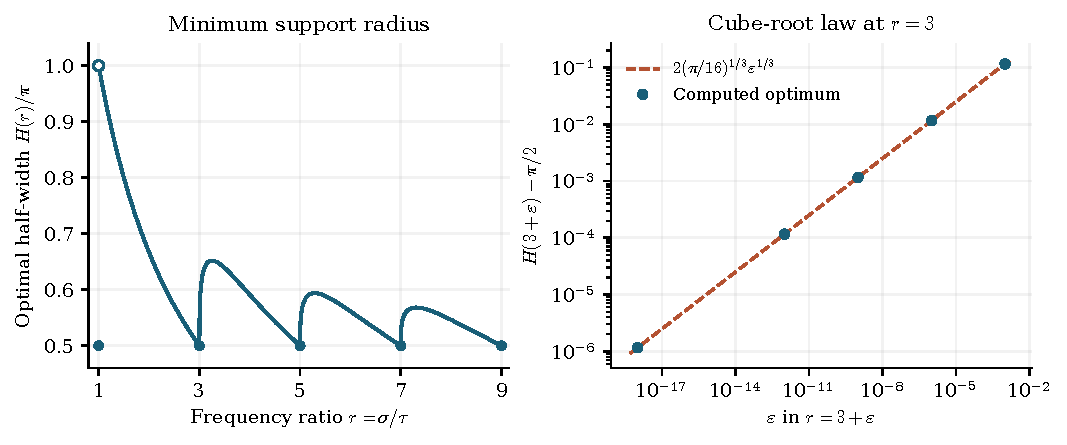
\includegraphics[width=\textwidth]{figures/resonance.pdf}
\caption{The minimum normalized half-width and its right-hand cusp near $r=3$.
The curves are numerical illustrations of the proved formulas. Left: the
solid value at $r=1$ imposes just one constraint; the open value is the limit
from two distinct frequencies. Right: the dashed line is the proved leading
term $2(\pi/16)^{1/3}\varepsilon^{1/3}$.}
\label{fig:resonance}
\end{figure}

The data include an illustrative filter for the first two numerically
computed zeta ordinates. It is not a certified computation of those zeros.
The mathematical filter theorem accepts any two specified positive real
frequencies, so its proof does not depend on that numerical example.

\section{A route to formal verification}
\label{sec:formalization}

No new Lean theorem is claimed to have been compiled. The included
\path{FORMALIZATION_PLAN.txt} separates the proof into reusable obligations.
For the branch result, finite truncation reduces the observations and target
to finite-dimensional vector spaces. The difficult mathematical interface is
the product-domination lemma, which uses a valued splitting field and the
multiplicativity of weighted Gauss valuation. After that interface, exact
distance, errors and erasures, and the tree recurrence are finite statements.
The componentwise saturation proof can be formalized independently by monic
polynomial division and Lagrange interpolation over $F((X))$.

For the filter result, one formalizes the scalar monotonicity arguments and
the nonnegative dual certificate first. A measure whose integral against a
continuous nonnegative function is zero is supported on its zero set; the
equality case then becomes a finite linear system. The cusp proof requires
uniform Taylor remainders and the two-sided scale comparison before dividing
by $u^3$ or $v^3$. A list of numerical samples cannot replace these obligations.

The source theorem and the new proofs therefore have distinct verification
statuses: the supplied development contains Lean proofs of its exported
RH/Dirichlet-GRH statements; this task inspected selected source files and
provides new conventional proofs with exact and numerical supporting checks.
It does not turn the new statements into Lean-verified theorems merely by
placing them beside that source.

\phantomsection
\addcontentsline{toc}{section}{References}
\begin{thebibliography}{12}
\small\raggedright
\bibitem{Source}
ProveIt contributors, \emph{Beyond the Riemann hypothesis for Dirichlet
$L$-functions: consequences, transfers and limits}, repository maintained by
V. Reshetnikov (2026). Snapshot in Section~\ref{sec:sources}.
\href{https://github.com/VladimirReshetnikov/ProveIt/tree/2a9f8e3ee74a1824d57546f0b1b4f1cef5df93d6/Analysis/GeneralizedRiemannHypothesis/Article}{Article and provenance};
\href{https://github.com/VladimirReshetnikov/ProveIt/blob/2a9f8e3ee74a1824d57546f0b1b4f1cef5df93d6/Analysis/GeneralizedRiemannHypothesis/Article/sections/lub.tex}{Lubin--Tate and recovery section};
\href{https://github.com/VladimirReshetnikov/ProveIt/blob/2a9f8e3ee74a1824d57546f0b1b4f1cef5df93d6/Analysis/GeneralizedRiemannHypothesis/Article/sections/rec.tex}{positive-filter section};
\href{https://github.com/VladimirReshetnikov/ProveIt/blob/2a9f8e3ee74a1824d57546f0b1b4f1cef5df93d6/Analysis/GeneralizedRiemannHypothesis/Article/sections/zer.tex}{prime-error section}.

\bibitem{Vendor}
ProveIt, vendored readable edition of \emph{grh-lean},
\href{https://github.com/VladimirReshetnikov/ProveIt/blob/2a9f8e3ee74a1824d57546f0b1b4f1cef5df93d6/Analysis/GeneralizedRiemannHypothesis/vendor/grh-lean/README.md}{vendor README};
\href{https://github.com/VladimirReshetnikov/ProveIt/blob/2a9f8e3ee74a1824d57546f0b1b4f1cef5df93d6/Analysis/GeneralizedRiemannHypothesis/vendor/grh-lean/grh/GUIDE.md}{upstream guide}.

\bibitem{LeanExports}
\emph{grh-lean} contributors,
\href{https://github.com/VladimirReshetnikov/ProveIt/blob/2a9f8e3ee74a1824d57546f0b1b4f1cef5df93d6/Analysis/GeneralizedRiemannHypothesis/vendor/grh-lean/grh/src/Statements.lean}{Statements.lean}
and
\href{https://github.com/VladimirReshetnikov/ProveIt/blob/2a9f8e3ee74a1824d57546f0b1b4f1cef5df93d6/Analysis/GeneralizedRiemannHypothesis/vendor/grh-lean/grh/src/Main.lean}{Main.lean},
same pinned snapshot.

\bibitem{LeanMechanism}
\emph{grh-lean} contributors,
\href{https://github.com/VladimirReshetnikov/ProveIt/blob/2a9f8e3ee74a1824d57546f0b1b4f1cef5df93d6/Analysis/GeneralizedRiemannHypothesis/vendor/grh-lean/grh/src/New/Reduction/MainInequality.lean}{MainInequality.lean},
\href{https://github.com/VladimirReshetnikov/ProveIt/blob/2a9f8e3ee74a1824d57546f0b1b4f1cef5df93d6/Analysis/GeneralizedRiemannHypothesis/vendor/grh-lean/grh/src/New/Reduction/OneSidedBound.lean}{OneSidedBound.lean},
\href{https://github.com/VladimirReshetnikov/ProveIt/blob/2a9f8e3ee74a1824d57546f0b1b4f1cef5df93d6/Analysis/GeneralizedRiemannHypothesis/vendor/grh-lean/grh/src/New/Determinant/Twist/LongForms.lean}{LongForms.lean},
same pinned snapshot.

\bibitem{LeanLocal}
\emph{grh-lean} contributors,
\href{https://github.com/VladimirReshetnikov/ProveIt/blob/2a9f8e3ee74a1824d57546f0b1b4f1cef5df93d6/Analysis/GeneralizedRiemannHypothesis/vendor/grh-lean/grh/src/Lib/CM/FormalGroup/InseparableDegree.lean}{InseparableDegree.lean},
same pinned snapshot.

\bibitem{Bhargava2009}
M. Bhargava, On $P$-orderings, rings of integer-valued polynomials, and
ultrametric analysis, \emph{J. Amer. Math. Soc.} 22 (2009), 963--993.
\href{https://doi.org/10.1090/S0894-0347-09-00638-9}{doi:10.1090/S0894-0347-09-00638-9}.

\bibitem{Amini2016}
O. Amini, \emph{Logarithmic tree factorials}, arXiv:1611.02142 (2016);
author's February 2017 draft.
\href{https://arxiv.org/abs/1611.02142}{arXiv record}.

\bibitem{MO}
\emph{Maximum number of roots of a monic degree-$d$ polynomial modulo $p^k$},
\href{https://mathoverflow.net/questions/515610/maximum-number-of-roots-of-a-monic-degree-d-polynomial-modulo-pk}{MathOverflow question 515610}.
Accessed 27 November 2026. A public research discussion, not a
peer-reviewed priority determination.

\bibitem{Gao}
S. Gao, \emph{A new algorithm for decoding Reed--Solomon codes},
\href{https://www.math.clemson.edu/~sgao/papers/RS.pdf}{author's paper}.

\bibitem{NASA1995}
Convolve, Inc., \emph{Minimizing Structural Vibrations with Input Shaping},
NASA-CR-189439 (January 1995), printed pp.\ 39--42, equations (15)--(16).
\href{https://ntrs.nasa.gov/api/citations/19950024365/downloads/19950024365.pdf}{NASA full report}.

\bibitem{Shaping1997}
W. Singhose, E. Crain, and W. Seering,
Convolved and simultaneous two-mode input shapers,
\emph{IEE Proceedings--Control Theory and Applications} 144 (1997), 515--520.
\href{https://doi.org/10.1049/ip-cta:19971439}{doi:10.1049/ip-cta:19971439}.
Bibliographic antecedent; its full text was not independently checked here.
\end{thebibliography}

\end{document}
